\documentclass[]{report}
\usepackage{pdfpages} 
\usepackage[utf8]{inputenc}
\usepackage[spanish]{babel}

\usepackage{cite} % para contraer referencias
% Title Page
\title{Protocolo de tesis}
\author{Efren López Jiménez}


\begin{document}
	
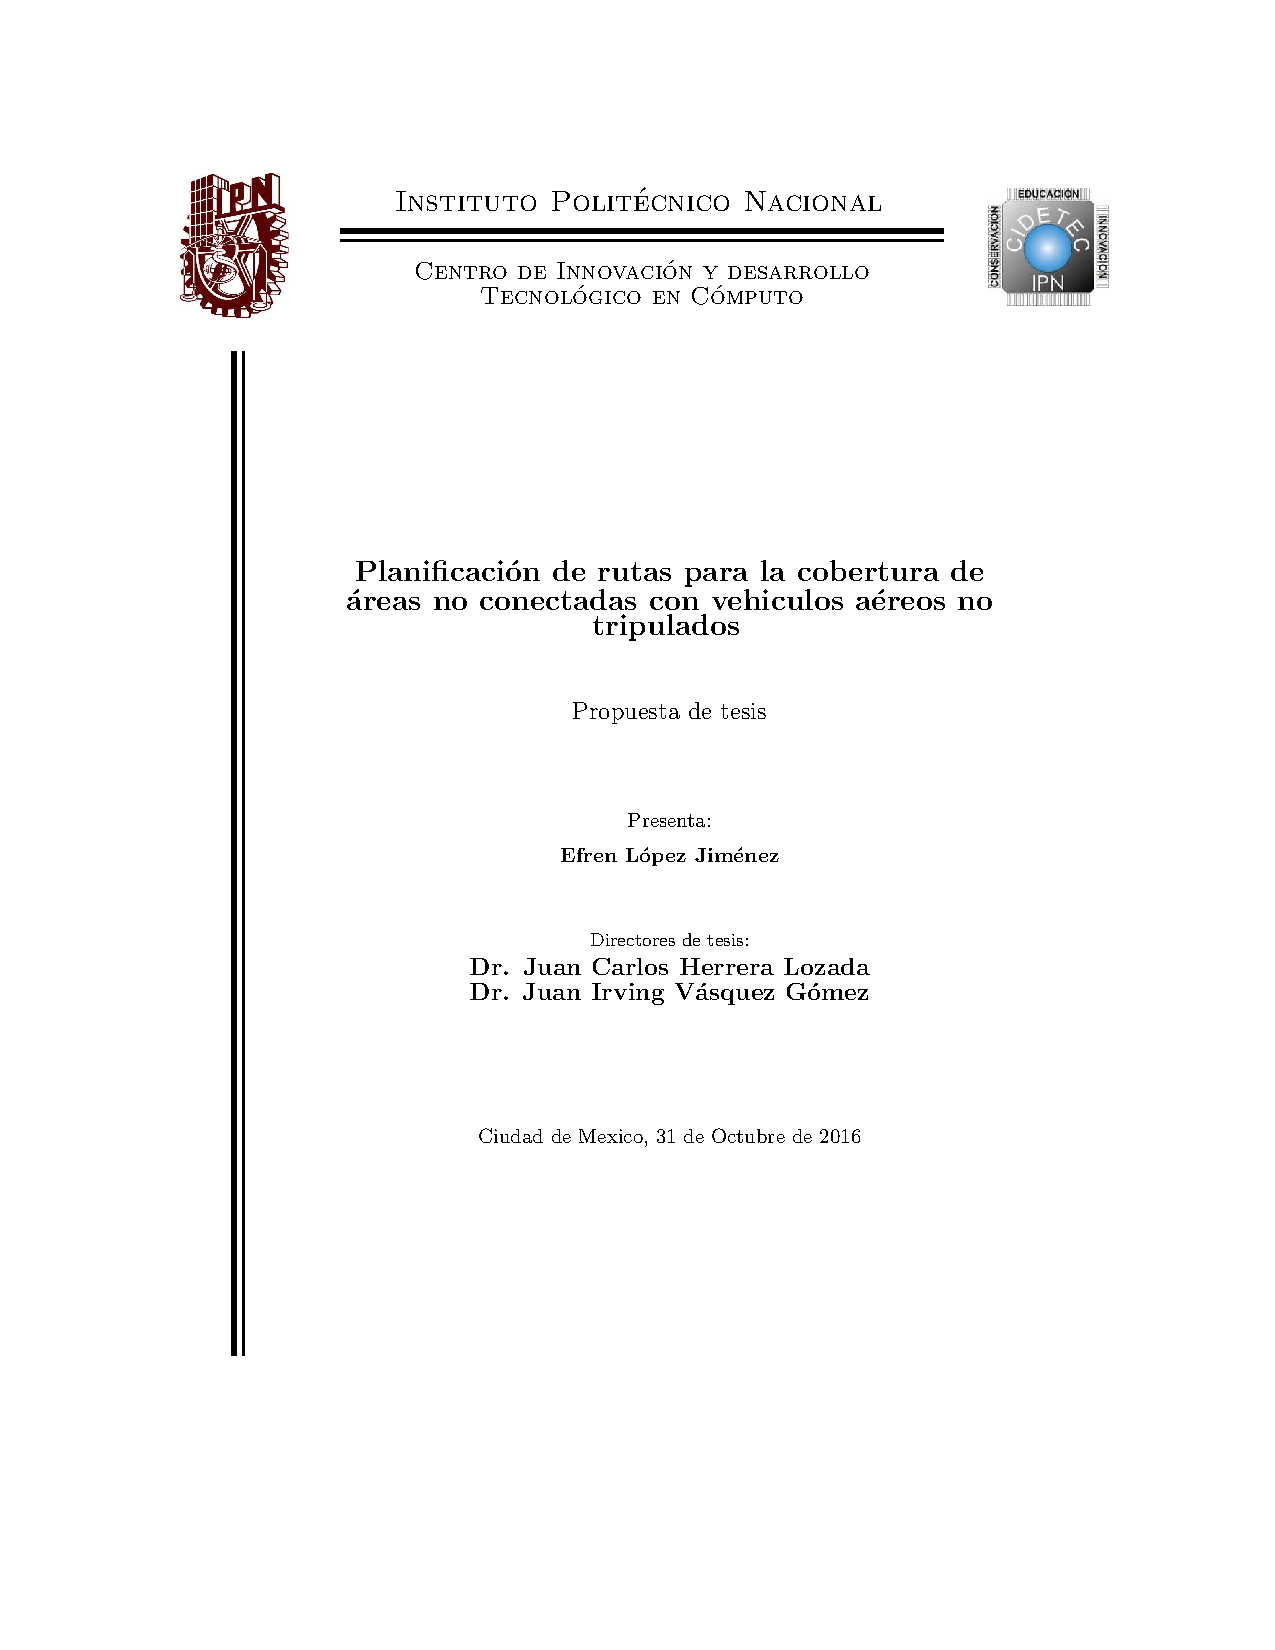
\includepdf[pages={1}]{portada.pdf}
	

\newpage\null\thispagestyle{empty}\newpage
	
%\maketitle

\begin{abstract}
	
La implementación de Vehículos aéreos no tripulados en diferentes sectores es  presente trabajo se presenta bajo la premisa de mejorar el aprovechamiento de los recursos que nos ofrece un vehículo aéreo no tripulado, debido a la importancia de  
\end{abstract}

\addtocontents{toc}{\hfill \textbf{Página} \par}
\tableofcontents

\chapter{Introducción}
La exploración de áreas,ha sido tratada y estudiada desde tiempos remotos, se ha intentado de diferentes maneras, por ejemplo con móviles terrestres, utilizando diferentes algoritmos, donde tienen un objetivo final, la exploración de un área en particular teniendo aplicaciones en diferentes áreas de investigación, por ejemplo robots contra incendios, robots de rescate, etc.
Durante los últimos años la importancia del uso de los UAV, ha impactado  el crecimiento y desarrollo de las Tecnologías aéreas ha sido exponencial, esto debido a que la mano del hombre ha reducido considerablemente en la manipulación de dichos robots.
La importancia de estudiar los dispositivos móviles en particular los dispositivos aéreos, empieza cuando se requiere explorar zonas de alta peligrosidad, o zonas complejas donde implica un riesgo al ser humano.
Uno de los grandes retos a enfrentar en el área de robótica con vehículos no tripulados, es la planificación de rutas conocidas o no conocidas, que nos permitan conocer o explorar un área independientemente de la utilidad o objetivo que se pretenda realizar. los experimentos pueden ser con obstáculos complejos o determinar un espacio en particular, la idea se genera a partir de la necesidad de reducir el tiempo de vuelo, cubriendo en su totalidad un área de interés en particular.
La batería de un vehículo aéreo, ha sido una limitante para el recorrido de un vehículo aéreo, gracias a esto se piensa en la reducción de tiempo de vuelo implementando nuevos algoritmos que nos permitan cubrir un área en menos tiempo, 

\section{Motivación}
Se han realizado trabajos e investigación con planificación de rutas con vehículos aéreos no tripulados en áreas convexas y de un polígono, este trabajo esta enfocada en la importancia de recorrer un área no conectada
La importancia del presente trabajo radica en implementar nuevas tecnologías en los diferentes sectores de servicio y productivo, por ejemplo en la agricultura, ha sido un área de oportunidad donde se requieren nuevas tecnologías para obtener información, datos de un terreno, por ejemplo medir la   debido a los rezagos tecnológico, siendo un sector fundamental para el desarrollo del país

\section{Problema}

Debido a la importancia de  obtener información de dichas terrenos o áreas de difícil acceso e características no conocidas  radica en la necesidad de cubrir un determinado área no convexa dado un conjunto de dos polígonos no conectados, minimizando el costo en función de la necesidad de obtener información necesaria para una determinada aplicación en dichas áreas, a fin de alguna aplicación en particular, como por ejemplo cubrir un área de cultivo para determinar estadísticas de mejoramiento de cultivo, nuevas técnicas de fertilización

\chapter{Trabajo Relacionado}

J.F. Araujo, P.B Sujit, J.B Sousa propone que la cobertura de un área involucra dos etapas: descomposición del área y la planificación de la trayectoria utilizando técnicas de barrido, para la planificación de rutas dentro de la superficie; la misión es en tiempo mínimo.\cite{1}\\
Anqi Xu, Chatavut Viriyasuthee, and Ioannis Rekleitis propone sobre  la estrategia en calcular una trayectoria a través de un ambiente con obstáculos, asegurando la cobertura completa minimizando la repetición de la trayectoria, con este algoritmo evita un conjunto de regiones con obstáculos de forma arbitraria, evitar sobre regiones previamente ya cubiertas e iniciando y terminando en la misma localización. \cite{2}
Eric Galceran, Marc Carreras hacen una revision exhaustiva 

\chapter{Propuesta}
La contribución de este trabajo es mejorar el rendimiento de la cobertura de un vehículo aéreo no tripulado,utilizando otros algoritmos que nos permitan mejorar el tiempo de recorrido y cumplir con la misión cargada en el mismo.
Ademas, se piensa utilizar un sistema embebido con el fin de procesar las imágenes obtenidas 



\section{Hipótesis}
Los trabajos previos relacionados con esta área de investigación aportan

\section{Objetivo General}
Desarrollar un algoritmo de planificación de rutas para cubrir una superficie.
\section{Objetivos Específicos}
\begin{itemize}
\item Realizar un estudio de diferentes algoritmos y seleccionar el mas adecuado.
\item Realizar un estudio de diferentes técnicas de planificación de rutas.
\item Implementación de un sistema embebido para el desarrollo de un algoritmo para la planificación de la ruta adecuada del UAV.
\item Validación del sistema implementado.
\item Análisis de un sistema embebido para la captura y procesamiento de imágenes
\end{itemize}
\section{Metodología}
La metodología que se va a utilizar estará determinada por etapas, el cual consiste de lo siguiente:


\subsection{Cronograma}

\begin{tabular}{|c|c|c|c|c|c|}
	\hline 
	& 1 Semestre  & 2 Semestre  & 3 Semestre  & 4 Semestre \\ 
	\hline 
	Actividad &  &  &  &  \\ 
	\hline
	Protocolo de defensa de tesis & ******* &  &  &  \\ 
	\hline 
	Diseño del experimento  &  &******  &  &  \\ 
	\hline
	Resultados &  &  &****  &  \\ 
	\hline
	Revisión de literatura &****  &****  &*****  &****  \\ 
	\hline 
	Defensa de Tesis &  &  &  &****  \\ 
	\hline  
\end{tabular} 

\chapter{Avances}

\chapter{Conclusiones}

\chapter {Referencias}
\bibliographystyle{plain}
\bibliography{bibliography}



\end{document}          
